\section{Convolutional Neural Network Classifier} \label{sec:CNN}
	\pagestyle{mario}
	\sectionauthor{M. Gini \& T. M. Hayden}

CNN is a more advanced architecture compared to a MLP network. Similarly to a MLP, it consists of an input as well as an output layer, as well as several hidden layers. The hidden layers typically consist of convolutional layers, pooling layers, fully connected layers and normalization layers. Due to that, CNN are usually much deeper than MLP networks.

However, CNN require significantly more computing power to train. Even though MATLAB supports training on the GPU, some quick maths reveal that our computational resources are insufficient for extensive parameter search of a CNN.

	
\subsection{Network Structure}

Since the number of hidden layers of a CNN can be quite large, even more hyperparameters could be explored than for an MLP. This takes unreasonable amounts of time. Therefore, this section only presents the final version of our CNN which is found through small trial-and-error tests. It consists of 16 layers which are summarized below.

\begin{itemize}
	\item \textbf{Input Layer}\\
	For a color image, the channel size is 3, corresponding to the RGB values. You do not need to shuffle the data because trainNetwork, by default, shuffles the data at the beginning of training.
	
	\item \textbf{Convolutional Units}\\
	This CNN possesses three convolutional units. A convolutional unit consists of several layers. The first layer is always the \textit{convolutional layer}. It has parameters for filter size and depth, which control the size and number of feature maps the layer is analyzing. This layer is followed by a \textit{batch normalization layer} which normalizes the activations and gradients propagating through a network, making network training an easier optimization problem.
	
	Then, a \textit{rectified linear unit} (ReLU) follows. This is a nonlinear activation function very commonly used in CNN.
	
	\item \textbf{Output Layer}\\
	The output layer consists of a softmax layer as described earlier together with a classification layer which simply chooses the class that obtained the highest prediction by the softmax layer.
	
\end{itemize}


Batch Normalization Layer Batch normalization layers normalize the activations and gradients propagating through a network, making network training an easier optimization problem. Use batch normalization layers between convolutional layers and nonlinearities, such as ReLU layers, to speed up network training and reduce the sensitivity to network initialization. Use BatchNormalizationLayer to create a batch normalization layer.

ReLU Layer The batch normalization layer is followed by a nonlinear activation function. The most common activation function is the rectified linear unit (ReLU). Use ReLULayer to create a ReLU layer.

Max-Pooling Layer Convolutional layers (with activation functions) are sometimes followed by a down-sampling operation that reduces the spatial size of the feature map and removes redundant spatial information. Down-sampling makes it possible to increase the number of filters in deeper convolutional layers without increasing the required amount of computation per layer. One way of down-sampling is using a max pooling, which you create using MaxPooling2DLayer. The max pooling layer returns the maximum values of rectangular regions of inputs, specified by the first argument, poolSize. In this example, the size of the rectangular region is [2,2]. The 'Stride' name-value pair argument specifies the step size that the training function takes as it scans along the input.

Fully Connected Layer The convolutional and down-sampling layers are followed by one or more fully connected layers. As its name suggests, a fully connected layer is a layer in which the neurons connect to all the neurons in the preceding layer. This layer combines all the features learned by the previous layers across the image to identify the larger patterns. The last fully connected layer combines the features to classify the images. Therefore, the OutputSize parameter in the last fully connected layer is equal to the number of classes in the target data. In this example, the output size is 10, corresponding to the 10 classes. Use FullyConnectedLayer to create a fully connected layer.


\subsection{Test Accuracy Results}

Here, the results of a few tests are presented.

\begin{figure}[h!]
	\centering
	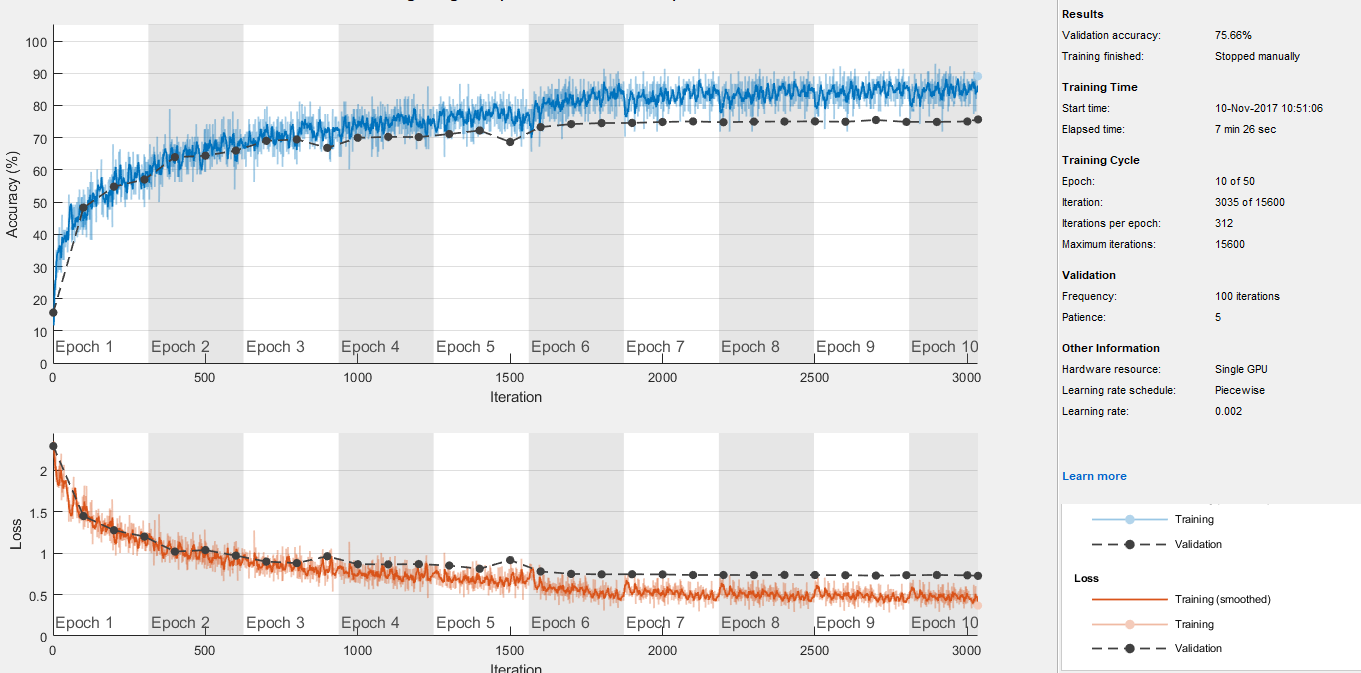
\includegraphics[width=\textwidth]{images/CNNTrain}
	\caption{MATLAB GUI for training CNN.}
	\label{fig:CNNTrain}
\end{figure}



    
